Para cumplir los objetivos establecidos en este proyecto, es necesario desarrollar un marco teórico que aborde temas importantes sobre el funcionamiento del dron Crazyflie 2.1 y sus componentes. Así como conocer la estructura de las herramientas de control disponibles para el uso del dron Crazyflie.


\section{Crazyflie 2.1 }
Los drones Crazyflie son plataformas de desarrollo aéreo de código abierto desarrollados por Bitcraze. Están diseñados principalmente para investigación, desarrollo y educación en ingeniería de control y robótica. Como se observa en la Figura \ref{fig:Crazyflie}, tienen un tamaño reducido, pero están equipados con una variedad de sensores que lo vuelven ideal para explorar algoritmos de control y otras aplicaciones. 
\begin{figure}[htbp]
	\centering
	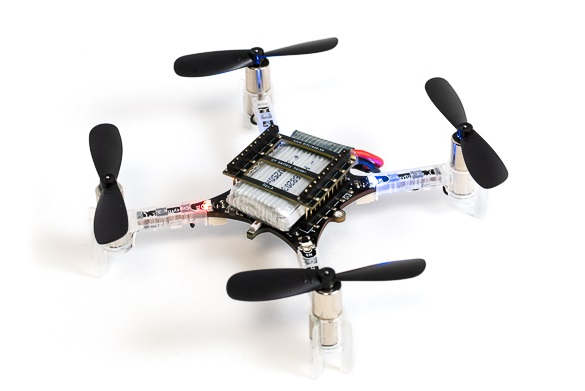
\includegraphics[width=0.45\textwidth]{Crazyflie}
	\caption{Dron Crazyflie 2.1 \cite{Crazyflie}.}
	\label{fig:Crazyflie}
\end{figure}
\\El Crazyflie 2.1 es un mini dron que pesa aproximadamente 27 gramos y tiene dimensiones generales de 92$\times$92$\times$29 mm. Su control se realiza mediante \textit{Bluetooth} o radiofrecuencia, lo que le permite ser controlado desde dispositivos móviles, así como desde sistemas operativos Windows, Mac OSX y Linux utilizando Crazyradio o Crazyradio PA. En cuanto a sus características eléctricas, el Crazyflie 2.1 dispone de una batería de litio-polímero (Li-Po) con modos desde 100 mA hasta 980 mA, que alimenta motores, microcontroladores y demás componentes. Utiliza un microcontrolador STM32F405 para el control de vuelo y un microcontrolador nRF51 para la comunicación inalámbrica. Está equipado con un acelerómetro/giroscopio de 3 ejes BMI088 y un sensor de presión de alta precisión BMP388, pero también permite la integración de otras placas de expansión para ampliar sus capacidades, con la restricción de que soporta una carga adicional de hasta 15 gramos que puede afectar el tiempo de vuelo debido al aumento de demanda de energía \cite{Crazyflie}. 

\section{Sistema de coordenadas de dron Crazyflie}
Los drones Crazyflie, al igual que la mayoría de los drones, utilizan la convención de sistema de coordenadas tridimensional ENU (\textit{East North Up}) para determinar su posición y orientación en el espacio. Como se observa en la Figura \ref{fig:Sistema_Crazyflie}, el dron tiene tres ejes principales de referencia: el eje X es horizontal y apunta hacia adelante, el eje Y es horizontal y apunta hacia la derecha y el eje Z es vertical y apunta hacia arriba. 

Por otro lado, la orientación del dron se describe en términos de ángulos de inclinación respecto a los ejes de referencia. El ángulo de balanceo (\textit{roll}) se refiere a la inclinación del dron hacia los lados en torno al eje X, el ángulo de cabeceo (\textit{pitch}) se refiere a la inclinación hacia adelante o hacia atrás en torno al eje Y, y el ángulo de guiñada (\textit{yaw}) se refiere a la rotación del dron en torno al eje Z. Según la documentación oficial de Bitcraze, estos ángulos siguen las siguientes reglas de rotación: \textit{roll} y \textit{yaw} rotan en sentido horario alrededor del eje al mirar desde el origen, mientras que \textit{pitch} rota en sentido antihorario alrededor del eje al mirar desde el origen \cite{Sistema_Crazyflie}.

\begin{figure}[htbp]
	\centering
	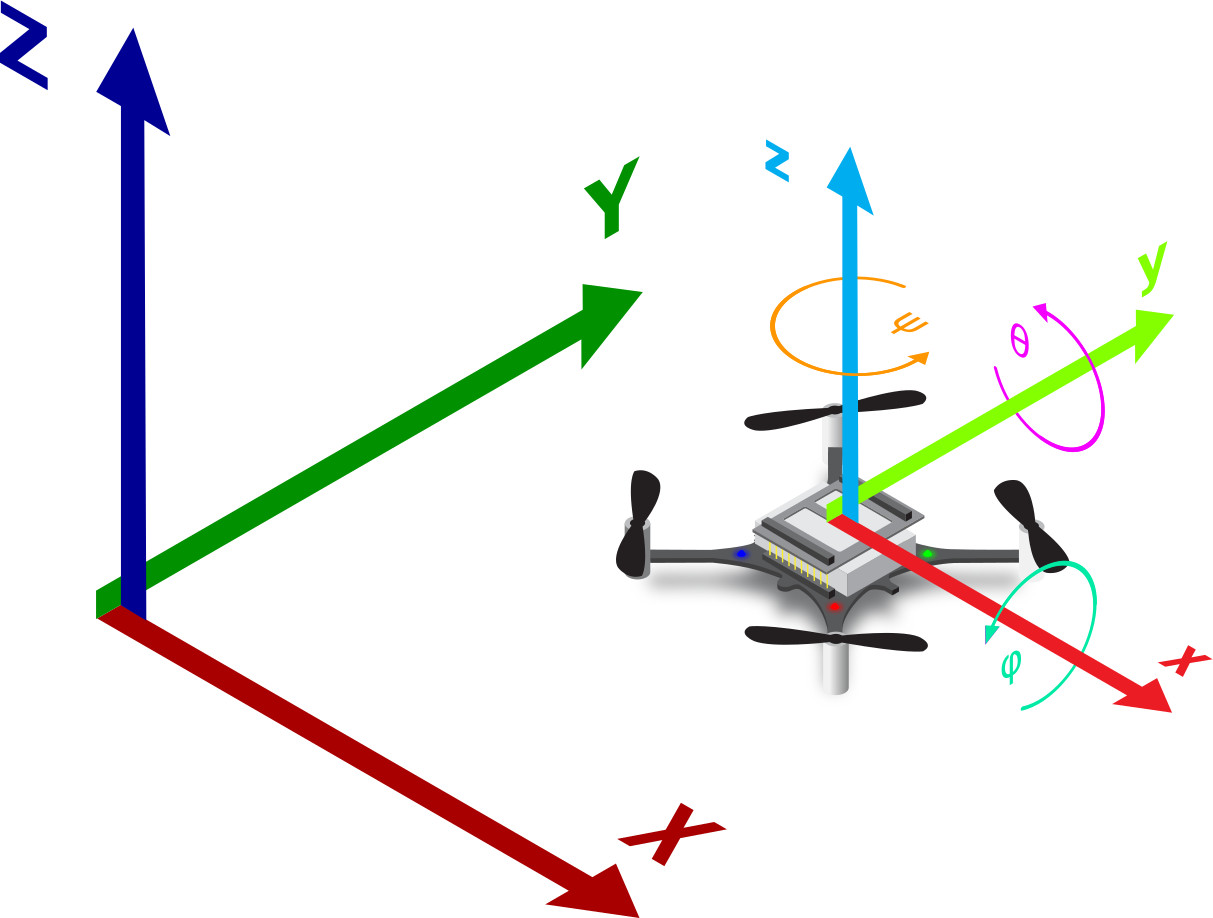
\includegraphics[width=0.6\textwidth]{Sistema_Crazyflie}
	\caption{Sistema de coordenadas de Crazyflie 2.1 \cite{Sistema_Crazyflie}.}
	\label{fig:Sistema_Crazyflie}
\end{figure}

\section{Comunicación inalámbrica de dron Crazyflie}
Los drones Crazyflie establecen una comunicación inalámbrica por medio del dispositivo Crazyradio, mostrado en la Figura \ref{fig:Crazyradio}. Esta comunicación se basa en un enlace de radiofrecuencia bidireccional que permite enviar comandos de control al dron y recibir datos en tiempo real sobre su posición, orientación y otros parámetros relevantes.

\begin{figure}[htbp]
	\centering
	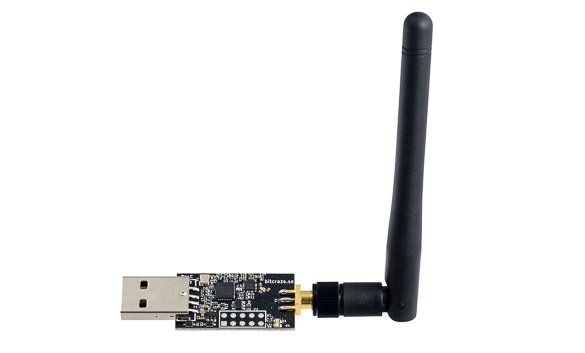
\includegraphics[width=0.47\textwidth]{Crazyradio}
	\caption{Dispositivo de comunicación inalámbrica Crazyradio \cite{Crazyradio}.}
	\label{fig:Crazyradio}
\end{figure}
\\ El Crazyradio es un transceptor de radio USB de código abierto, baja latencia y largo alcance. Funciona en la banda de 2.4 GHz con un rango de transmisión de hasta 1 km (en condiciones ideales) gracias a su amplificador de radio de 20 dBm. Está basado en el microcontrolador nRF24LU1 de Nordic Semiconductor y se comunica por medio del protocolo “\textit{Enhanced ShockBurst}” compatible con los microcontroladores nRF24L01p, nRF51 y nRF52. En una capa de nivel más alto, utiliza el protocolo de paquetes CRTP para comunicarse con el Crazyflie y poder actualizar el \textit{firmware}, enviar comandos y recibir información de los drones. Dependiendo del sistema operativo, es necesario instalar controladores o realizar configuraciones específicas \cite{Crazyradio}.

\section{Placa de expansión Flow Deck}
El Flow Deck es una placa de expansión diseñada específicamente para mejorar las capacidades de percepción de los drones Crazyflie. Esta placa funciona como un sistema de posicionamiento para el dron, otorgándole la capacidad de comprender su posición y velocidad en un entorno tridimensional. 

\begin{figure}[htbp]
	\centering
	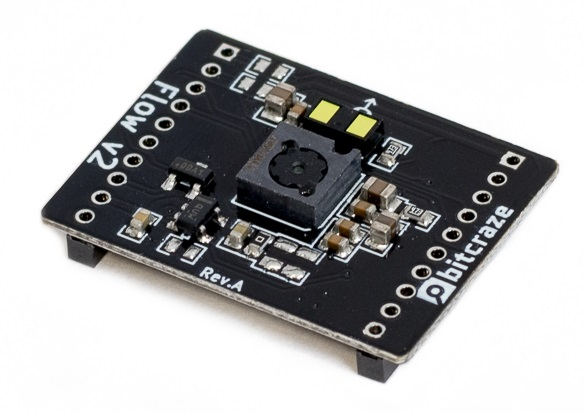
\includegraphics[width=0.37\textwidth]{FlowDeck}
	\caption{Placa de expansión Flow Deck v2 \cite{FlowDeck}.}
	\label{fig:FlowDeck}
\end{figure}

La placa Flow Deck, mostrada en la Figura \ref{fig:FlowDeck}, tiene un peso aproximado de 1,6 gramos y dimensiones generales de 21$\times$28$\times$4 mm. Para integrarlo se requiere actualizar el \textit{firmware} del Crazyflie a su última versión y montarlo en la parte inferior del dron. \cite{FlowDeck}. 

Utiliza el sensor de medición de distancias VL53L1x para determinar su altura junto al sensor de flujo óptico PMW3901 que mide movimientos horizontales sobre la superficie mediante odometría visual. Como se observa en la Figura \ref{fig:Funcionamiento_FlowDeck}, la combincación de información obtenida de ambos sensores permite al dron hacer una estimación de su posición en un entorno tridimensional.

\begin{figure}[htbp]
	\centering
	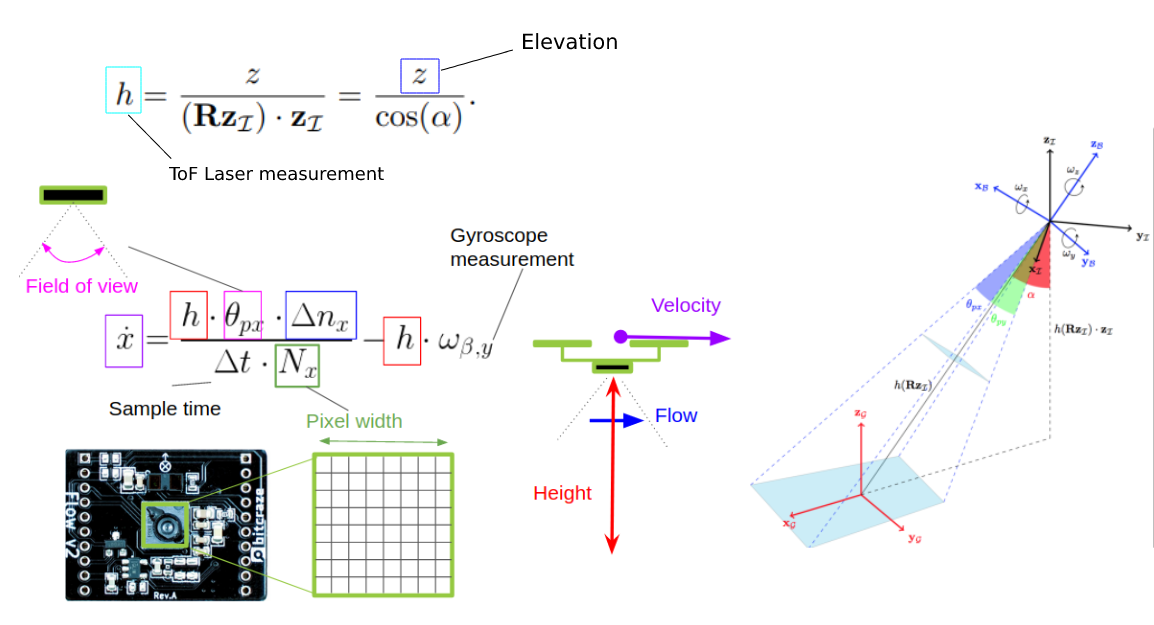
\includegraphics[width=0.75\textwidth]{Funcionamiento_FlowDeck}
	\caption{Funcionamiento de la placa Flow Deck y ecuación de estimación de posición \cite{Funcionamiento_FlowDeck}.}
	\label{fig:Funcionamiento_FlowDeck}
\end{figure}

\section{Odometría visual}
Odometría visual es un método que permite estimar el movimiento de un agente robótico utilizando infomación extraída a partir de imágenes capturadas por cámaras. Esta técnica de estimación de posición se basa en el análisis de una secuencia de imágenes para identificar y rastrear rasgos visuales distintivos. Tal como se muestra en la Figura \ref{fig:Optical_flow}, se realiza un seguimiento de los rasgos de fotograma a fotograma y el resultado es la distancia que la entidad se ha movido desde el fotograma anterior \cite{Persson2022_book}.

\vspace{0.3cm} % Espacio después de la imagen
\begin{figure}[htbp]
	\centering
	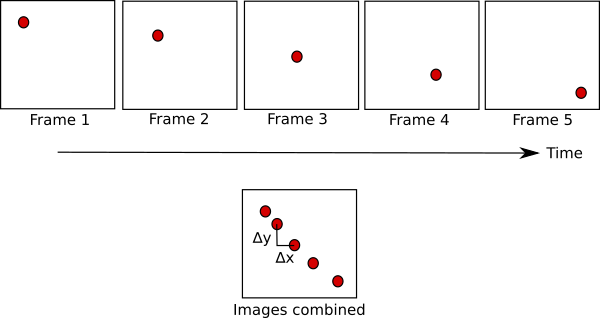
\includegraphics[width=0.55\textwidth]{Optical_flow}
	\caption{Diagrama de flujo óptico para estimación de posición con odometría visual \cite{Flujo_optico}.}
	\label{fig:Optical_flow}
\end{figure}

Este método resulta particularmente útil para entornos donde otras formas de localización no son viables o precisas, como en interiores o áreas con estructuras complejas. 

Como se mencionó con anterioridad, el sensor PMW3901 en la placa Flow Deck utiliza odometría visual para estimar las distancias desplazadas por rasgos distintivos en las imágenes capturadas. Esta información, junto con las mediciones de altura del sensor de distancia  VL53L1x, son combinadas en la ecuación de la Figura \ref{fig:Funcionamiento_FlowDeck} para estimar el movimiento del dron relativo a su punto de partida \cite{Funcionamiento_FlowDeck}.

 \section{Sensor de flujo óptico PMW3901}
PMW3901 es un sensor de flujo óptico desarrollado por Pixart Imaging, ampliamente utilizado en aplicaciones de robótica para estimar movimiento. Resulta de particular interés debido a que forma parte de la placa de expansión Flow Deck de Bitcraze y es el responsable de darle sentido de posición bidimensional (en los ejes X-Y) a los drones Crazyflie. Dentro de sus detalles técnicos, dispone un microcontrolador de bajo consumo que determina internamente el flujo óptico con algoritmos de odometría visual, proporcionando posición con base en diferencias en pixeles entre fotogramas. Opera con un voltaje que varía entre 1.8 y 2.1 V. Se comunica por medio de una interfaz SPI de 4 hilos que opera a 2 MHz, transmitiendo datos de movimiento almacenados en registros de 16 bits. Tiene un rango de operación desde 80 mm hasta el infinito y cuenta con una tasa de fotogramas de 121 FPS, detectando movimientos de hasta 7.4 radianes por segundo. Está encapsulado en un paquete \textit{chip-on-board} de 28 pines, lo que permite su integración en distintas aplicaciones \cite{PMW3901_datasheet}.

\section{Sensor de medición de distancias VL53L1x}
VL53L1x es un sensor de medición de distancias desarrollado por STM electronics. La placa de expansión Flow Deck tiene integrado este sensor para proporcionar sentido de altura de vuelo (eje Z) a los drones Crazyflie. En cuanto a sus especificaciones técnicas, el VL53L1x está basado en la tecnología de tiempo de vuelo (\textit{Time-of-Flight}, ToF) que permite medir el tiempo que tarde un pulso de luz en reflejarse desde un objeto y volver al sensor, proporcionando una medida precisa de la distancia del objeto. El sensor funciona emitiendo un láser invisible de 940 nm y utiliza una matriz de recepción SPAD (diodo de avalancha de fotón único) para detectar la luz reflejada, ofreciendo un campo de visión típico de 27 grados. Incluye un microcontrolador de bajo consumo que permite una medición de distancia de hasta 4 metros con una frecuencia de hasta 50 Hz y se comunica por medio de una interfaz I2C que soporta velocidades de hasta 400 kHz \cite{VL53L1x_datasheet}.

\newpage
\section{Librería en Python para Crazyflie: cflib}
La librería cflib es una herramienta en Python desarrollada por Bitcraze para facilitar la comunicación y control del dron Crazyflie. Esta librería proporciona una API robusta que permite implementar distintas operaciones en el dron, que van desde vuelo autónomo hasta la gestión y recopilación de lecturas de sensores. Además, cflib simplificia la interacción con el \textit{hardware} a través de comandos y funciones de alto nivel. La librería es asíncrona y se basa en devoluciones de llamada para eventos. Sin embargo, existen contenedores síncronos para clases seleccionadas que crean una API síncrona encapsulando las clases asíncronas \cite{Crazyflie_Python}.

\subsection{Estructura de la librería}
\subsubsection{Identificador uniforme de recursos (URI)}
Todos los enlaces de comunicación se identifican mediante una dirección URI estructurada con el formato: \textbf{InterfaceType://InterfaceId/InterfaceChannel/InterfaceSpeed}

Los tipos de interfaz actualmente disponibles con la estructuras de formato adecuada son los siguientes:
\begin{itemize}
	\item \textbf{radio://0/10/2M:} Interfaz de radio, dongle USB número 0, canal de radio 10 y radio velocidad 2 Mbit/s
	\item \textbf{debug://0/1:} Interfaz de depuración, id 0, canal 1
	\item \textbf{usb://0:} Cable USB a puerto microusb, id 0
	\item \textbf{serial://ttyAMA0:} Puerto serie, id ttyAMA0
	\item \textbf{tcp://tcp-1.local:300:} Conexión de red TCP, Nombre: tcp-1.local, puerto 300
\end{itemize}

\subsubsection{Variables y parámetros}
En la librería Crazyflie, tanto las variables de registro como los parámetros son fundamentales para monitorear y controlar el dron en tiempo real. Ambas se agrupan y acceden de manera estructurada siguiendo la misma convención de nombres: grupo.nombre.

\begin{itemize}
	\item \textbf{Variables:} Las variables de registro se utilizan para supervisar continuamente datos del dron. Se configuran para que el \textit{firmware} envíe estos datos al host a intervalos regulares.
	\item \textbf{Parámetros:} Los parámetros permiten leer y escribir configuraciones en el \textit{firmware} durante la ejecución. Son útiles para modificar ajustes que no cambian constantemente, como los valores de controladores PID o el resultado de las autocomprobaciones. 
\end{itemize}

\subsection{Módulos}
La librería está organizada en distintos módulos que permiten al usuario acceder a funcionalidades específicas del dron. Estos módulos completan la estructura de la librería cflib, proporcionando una API robusta para controlar, gestionar y optimizar el uso del dron Crazyflie en distintos entornos.

\begin{itemize}
	\item cflib
	\begin{itemize}
		\item Bootloader
		\item CPX
		\item Crazyflie
		\item CRTP
		\item Drivers
		\item Localization
		\item Positioning
		\item Utils
	\end{itemize}
\end{itemize}

\subsubsection{Módulo Bootloader}
El módulo Bootloader es responsable de gestionar el proceso de actualización del \textit{firmware} del dron Crazyflie. Este módulo proporciona las herramientas necesarias para realizar una actualización segura, tanto a través de interfaces USB como de radio. Utiliza el protocolo \textit{bootloading} del Crazyflie para coordinar la transferencia de datos, gestionar las versiones y garantizar la correcta escritura en la memoria flash del dron \cite{Bootloader}. 

\subsubsection{Módulo CPX}
El módulo CPX proporciona un conjunto de herramientas para gestionar la comunicación entre el dron Crazyflie y otras plataformas mediantes distintos mecanismos de transferencia, como \textit{sockets} TCP y UART. Permite el intercambio de datos entre el dron y dispositivos externos \cite{CPX}.

\subsubsection{Módulo Crazyflie} 
El módulo Crazyflie es el núcleo de la librería y posee una amplia colección de herramientas diseñadas para controlar al dron Crazyflie. Este módulo ofrece una interfaz para interactuar con el dron, permitiendo el control de vuelo, la gestión de parámetros, la adquisición de datos y otras funciones. Está compuesto por la clase principal Crazyflie y otras clases auxiliares que gestionan diferentes aspectos del control del dron, como la conexión y la configuración \cite{Crazyflie_module}.

\subsubsection{Módulo CRTP}
El módulo CRTP (\textit{Crazy Real-Time Protocol}) conforma al protocolo de comunicación entre el controlador y el dron Crazyflie. Este protocolo es el responsable de estructurar los paquetes de datos en la comunicación con el dron, permitiendo una interacción a nivel bajo entre el \textit{hardware} y el \textit{software}. Además, dispone de las herramientas necesarias para configurar y gestionar las conexiones, asegurando una comunicación segura y eficiente \cite{CRTP}.

\subsubsection{Módulo Drivers}
El módulo de Drivers contiene las implementaciones necesarias para la interacción con el \textit{hardware} del dron Crazyflie. Estas herramientas permiten gestionar las distintas interfaces de comunicación y control entre el \textit{software} y el \textit{hardware}. Dentro del módulo Drivers se encuentran componentes que habilitan la conexión física mediante interfaces como USB y radio, garantizando una transferencia de datos segura y eficiente \cite{Drivers}.

\subsubsection{Módulo Localization}
El módulo Localization permite obtener y gestionar datos relacionados con la posición y localización del dron Crazyflie. A través de este módulo, el usuario puede utilizar sistemas de localización externa, como cámaras o estaciones de anclaje, para rastrear el movimiento del dron con precisión en tiempo real \cite{Localization}.

\subsubsection{Módulo Positioning}
El módulo Positioning se encarga de gestionar los sistemas de posicionamiento de Crazyflie. Incluye algoritmos y configuraciones para obtener la posición precisa del dron a través de sensores de posicionamiento \cite{Positioning}.

\subsubsection{Módulo Utils}
El módulo Utils contiene utilidades generales y herramientas de apoyo que facilitan el desarrollo de aplicaciones con el dron Crazyflie. Este módulo incluye funciones para el manejo de errores, herramientas de depuración y otras funciones auxiliares necesarias para mejorar la eficiencia y fiabilidad del desarrollo \cite{Utils}.

\vspace{0.5cm} % Espacio después de la imagen 
Los módulos anteriormente presentados conforman en totalidad a la librería cflib en Python y cada uno otroga funcionalidades específicas a la libería. Sin embargo, por la finalidad de este trabajo de graduación, algunos módulos presentan mayor relevancia que otros. En especial, los módulos Crazyflie y CRTP resultan particularmente importantes.

\newpage
\section{Módulo Crazyflie}
El módulo Crazyflie es relevante porque centraliza todas las operaciones esenciales para interacturar y controlar el dron. Coordina la interacción con el resto de módulos para formar una interfaz simple capaz de ejecutar funcionalidades específcias. Gracias a este módulo, es posible realizar tanto operaciones báscias como avanzadas con el dron Crazyflie.

\begin{itemize}
	\item \textbf{Clase principal crazyflie}
	\vspace{0.1cm} % Espacio después de la imagen 
	\\Es la clase que centraliza las operaciones necesarias para controlar el dron Crazyflie. Actúa como la interfaz directa entre el usuario y el dron, gestionando la conexión, el envío de comandos, el registro de datos y la configuración de parámetros. Además, la clase Crazyflie instancia y coordina varias clases auxiliares que facilitan tareas específicas. % (en \_\_init\_\_.py)
\end{itemize}

\begin{itemize}
	\item \textbf{Clases secundarias} 
	\begin{itemize}
		\item \textbf{appchannel:} Facilita la comunicación personalizada entre el dron y aplicaciones externas a través de un canal de aplicaciones.
		\item \textbf{commander:} Controla el movimiento y los comandos de vuelo del dron.
		
		\item \textbf{console:} Proporciona una interfaz para interactuar con la consola del dron, donde se pueden visualizar mensajes del \textit{firmware} del dron en tiempo real.
		
		\item \textbf{extpos:} Maneja la información de posicionamiento externo del dron, generalmente a través de sistemas de localización como cámaras externas.
		
		\item \textbf{high\_level\_commander:} Permite controlar el dron de manera autónoma, con comandos de alto nivel, como trayectorias predefinidas, despegue y aterrizaje.
		
		\item \textbf{localization:} Maneja los aspectos relacionados con la localización del dron Crazyflie, ayudando a rastrear su posición en el espacio.
		
		\item \textbf{log:} Gestiona el registro de datos del dron, como el estado de los sensores.
		
		\item \textbf{param:} Gestiona los parámetros configurables del dron, como la calibración de sensores y ajustes de vuelo.
		
		\item \textbf{plataformservice:} Gestiona la interacción entre el \textit{hardware} y el \textit{software} del dron, facilitando la integración de diferentes plataformas.
		
		\item \textbf{swarm:} Maneja la coordinación de múltiples drones Crazyflie, permitiendo controlarlos simultáneamente como un enjambre.
		
		\item \textbf{syncCrazyflie:} Proporciona una interfaz síncrona para la clase principal Crazyflie, facilitando la escritura de scripts secuenciales.
		
		\item \textbf{syncLogger:} Permite sincronizar el registro de datos de vuelo para garantizar la consistencia y precisión de los datos recolectados durante el vuelo.
		
		\item \textbf{toc:} Almacena un índice de las variables y parámetros disponibles en el dron, que pueden ser registrados o modificados.
		
		\item \textbf{toccache:} Almacena en caché las Tablas de Contenidos (TOC) del dron, optimizando la recuperación de datos y parámetros para evitar su descarga en cada nueva conexión.
	\end{itemize}
\end{itemize}

\newpage
\section{Módulo CRTP}
CRTP es el protocolo de empaquetamiento de datos utilizado para comunicarse con los drones Crazyflie. Este protocolo estructura los paquetes de información para dirigirlos a funcionalidades específicas del dron como el registro de datos, control de movimiento y parámetros de configuración.
 
La comunicación con Crazyflie se implementa como una pila de capas independientes. En la base se encuentra el medio físico (radio o USB), seguido por el enlace que garantiza la transmisión segura y ordenada de paquetes. Encima de esto está CRTP que maneja información de puerto y canal para dirigir los paquetes de datos a los distintos subsistemas del Crazyflie. Por último, los subsistemas implementan las funcionalidades del dron, controladas a través de CRTP.

Cada paquete CRTP incluye un número de puerto, un número de canal y una carga útil. Los puertos oscilan entre 0 y 15 y los canales entre 0 y 3, con la carga útil limitada a 31 bytes. Estos metadatos permiten dirigir los paquetes a los subsistemas correctos y las funcionalidades específicas dentro del Crazyflie \cite{Crazyflie_CRTP}.

El módulo dentro de la libería se ecuentra estructurado en submódulos con funcionalidades espcíficas:

\begin{itemize}
	\item \textbf{Submódulos}
	\vspace{0.1cm} 
	\begin{itemize}
		\item \textbf{cflib.crtp.crtpstack:} Administra el flujo de paquetes entre el dron y el controlador.
	\end{itemize}
	
	\begin{itemize}
		\item \textbf{cflib.crtp.exceptions:} Maneja los errores de comunicación CRTP, como pérdida de paquetes o tiempos de espera.
	\end{itemize}
	
	\begin{itemize}
		\item \textbf{cflib.crtp.pcap:} Captura paquetes CRTP para depuración y análisis.
	\end{itemize}
	
	\begin{itemize}
		\item \textbf{cflib.crtp.prrtdriver:} Implementa el PRRT para garantizar la entrega fiable de datos mediante retransmisiones.
	\end{itemize}
	
	\begin{itemize}
		\item \textbf{cflib.crtp.radiodriver:} Gestiona la comunicación inalámbrica por radio con el dron.
	\end{itemize}
	
	\begin{itemize}
		\item \textbf{cflib.crtp.serialdriver:} Maneja la comunicación por conexiones serie.
	\end{itemize}
	
	\begin{itemize}
		\item \textbf{cflib.crtp.tcpdriver:} Gestiona las conexiones TCP/IP.
	\end{itemize}
	
	\begin{itemize}
		\item \textbf{cflib.crtp.udpdriver:} Gestiona las conexiones UDP.
	\end{itemize}
	
	\begin{itemize}
		\item \textbf{cflib.crtp.usbdriver:} Administra la comunicación por puerto USB.
	\end{itemize}
\end{itemize}